\documentclass[tikz]{standalone}
\usepackage{tikz}
\usepackage{setspace}
\usepackage[UTF8]{ctex}
\usetikzlibrary{fit}
\usetikzlibrary{shapes}
\usetikzlibrary{backgrounds} 
\begin{document}
	\begin{spacing}{0.7}
		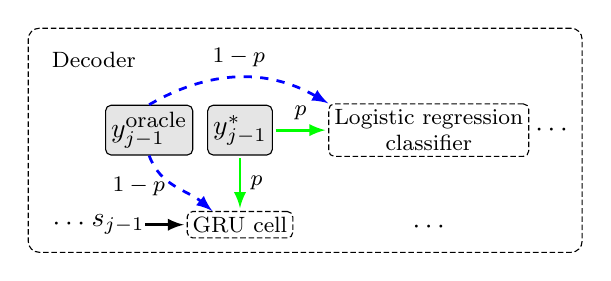
\begin{tikzpicture}
			\node[draw,fill=gray!20,rounded corners=2pt,inner sep=2pt, align=center,minimum height=1.8em] (oracle)at (0,0){$y_{j-1}^{\textrm{\footnotesize oracle}}$};
			\node[anchor=west,draw,fill=gray!20,rounded corners=2pt,inner sep=2pt, align=center,minimum height=1.8em](truth) at ([xshift=0.5em]oracle.east){$y_{j-1}^{*}$};
			\node[anchor=west,draw,rounded corners=2pt,inner sep=2pt, align=center,dash pattern=on 2pt off 1pt,minimum height=1.8em,font=\footnotesize](logit) at ([xshift=2em]truth.east){Logistic regression \\ classifier};
			\node[anchor=north,draw,rounded corners=2pt,inner sep=2pt, align=center,dash pattern=on 2pt off 1pt,font=\footnotesize](gru) at ([yshift=-2em]truth.south){GRU cell};
			\node[anchor=east,inner sep=0pt](s) at ([xshift=-1.5em]gru.west){$s_{j-1}$};

		\draw[-latex,color=green, line width=1pt] ([yshift=-0.1em]truth.south) -- node[color=black,right]{\footnotesize $p$} ([yshift=0.1em]gru.north);
		\draw[-latex,color=green, line width=1pt] ([xshift=0.1em]truth.east) -- node[color=black,above]{\footnotesize $p$} ([xshift=-0.1em]logit.west);
		\draw[-latex,dashed,color=blue,line width=1pt,out=30,in=150] (oracle.north) to node[color=black,above]{\footnotesize $1-p$}(logit.north west);
		\draw[-latex,dashed,color=blue,line width=1pt,out=-70,in=140] (oracle.south) to node[color=black,left]{\footnotesize $1-p$}([xshift=-1em]gru.north);
		\draw[-latex,line width=1pt] (s.east) -- ([xshift=-0.1em]gru.west);

		\node[anchor=east,inner sep=0pt] (o1) at ([xshift=-0.2em]s.west){$\cdots$};
		\node[anchor=north,inner sep=0pt] (o2) at ([yshift=-2.3em]logit.south){$\cdots$};
		\node[anchor=west,inner sep=0pt] (o3) at ([xshift=0.2em]logit.east){$\cdots$};
		\node[anchor=south] (decoder) at ([xshift=-2em,yshift=1em]oracle.north){\footnotesize Decoder};

		%background
    	\begin{pgfonlayer}{background}
        	\node [draw,rectangle,inner sep=0.5em,rounded corners=4pt,dash pattern=on 2pt off 1pt] [fit = (decoder)(gru) (o3)] (box0) {};
    	\end{pgfonlayer}
		\end{tikzpicture}
	\end{spacing}
\end{document} 